\chapter{Introduction}
\section{The course}
										
The main goals in this course are to experience and learn how to work on a 
development project as a team. In addition, the team has to answer to a 
customer, as software development companies often do, which stands out from 
other projects in the past. This is an advanced course and it is expected that 
knowledge obtained from previous courses is used, especially the development 
courses such as Informatics, Project I and the collaborative System Development 
project. \\

The group has an appointed guidance counselor as well as a customer. The 
counselor will be available for answering questions regarding the project 
management in general, and push the group to reflect on its decisions and 
review the work done. Status reports will be delivered regularly, so the 
counselor can stay up-to-date with the work in the group. \\

During the course, several project reports are scheduled for delivery; the 
preliminary project report, the mid-term project report and the final project 
report. Working on and delivering these reports will help in the planning and 
development of the project, and feedback will be given from the counselor. The 
grading of the project will take the final project report into consideration, 
as well as the final product.\\

\section{The team}
The team consists of six students of Informatics at NTNU:\\
\\
\textbf{Stian Aurheim}
\begin{itemize} \setlength{\itemsep}{0cm}\setlength{\parskip}{0cm}
	\item Third year bachelor in Informatics
	\item Main experience in Java. Some experience in Python, PHP, HTML, 
		  JavaScript 
\end{itemize}
\textbf{Jens Even Berg Blomsøy}
\begin{itemize} \setlength{\itemsep}{0cm}\setlength{\parskip}{0cm}
	\item Third year bachelor in Informatics
	\item Programming languages worked with: Java, Python.
	\item Main knowledge in System Development, system architecture and 
		  system documentation.
\end{itemize}
\textbf{Jørgen Foss Eri}
\begin{itemize} \setlength{\itemsep}{0cm}\setlength{\parskip}{0cm}
	\item Third year bachelor in Informatics
	\item Experience with Java, Python, JavaScript/HTML5/CSS3 and general web development
\end{itemize}
\textbf{Jim Frode Hoff}
\begin{itemize} \setlength{\itemsep}{0cm}\setlength{\parskip}{0cm}
	\item Third year bachelor in Informatics
	\item Programming languages worked with: Java, Python, PHP, JavaScript
		  and general web development
\end{itemize}
\textbf{Adrian Arne Skogvold}
\begin{itemize} \setlength{\itemsep}{0cm}\setlength{\parskip}{0cm}
	\item Third year bachelor in Informatics
	\item Programming languages worked with: Java, C\#, Oz, Actionscript
\end{itemize}
\textbf{Sindre Svendsrud}
\begin{itemize} \setlength{\itemsep}{0cm}\setlength{\parskip}{0cm}
	\item Third year bachelor in Informatics 
	\item Experience with Java, Python and C++
\end{itemize}

\section{Problem description} 

The customer has developed a paper prototype [Figure ~\ref{fig:paperPrototype}] 
of a board game called Don’t Panic. The game is designed to help crisis personell 
make the right decisions during a crisis in a city. It is a turn based, 
collaborative multiplayer strategy game where the players have to take actions to stop the 
inhabitants from panicking. After the game is finished, an expert will review 
the actions with the players to evaluate whether their choices were sound. 
\\
Our customer wants an electronic version of the board game. The electronic 
board game should maintain the social aspect (both physical and verbal) of a 
regular board game. In addition, a replay function will be added, to make it 
easy for the expert to review the game with the different players. The 
physical version of the board game takes a lot of work setting up and 
maintaining, as it is time consuming to move the pieces and update the panic 
levels. The electronic version will automate all of this.
\\

\begin{figure}[H]
  \centering
    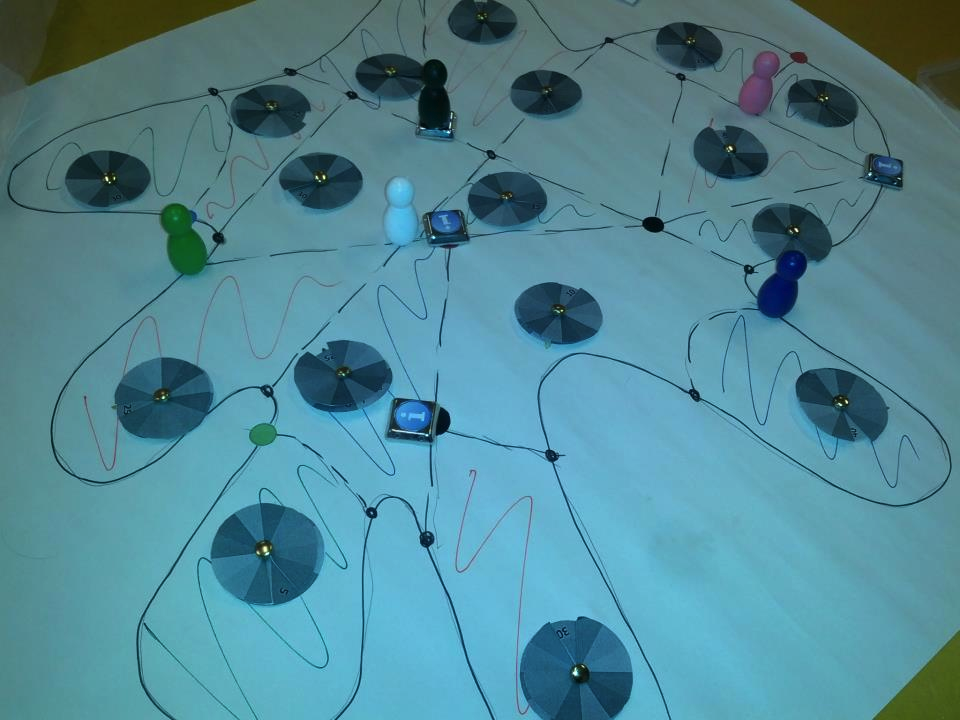
\includegraphics[width=1.0\textwidth]{img/paperprototype}
  \caption{Picture of the paper prototype} 
			% complete with colored zones, 
			% circular panic gauges, nodes, information centers, barricades 
			% and players 
  \label{fig:paperPrototype}
\end{figure}


\section{Constraints}

Only a few of us have some past experience with HTML5 and JavaScript\\
The game is to be completed within one semester (21 January - 27 May)

\section{Customer and supervisor}
The customer for this project is Ines Di Loreto, a researcher in the Department 
of Computer \& Information Science at NTNU. The supervisor assigned for this 
project is Mohsen Anvaari, a PhD candidate in the same department.




